\subsection{Applikation}
\label{subs:applikation}

Anforderungen aus \autoref{chap:anforderungen}, welche die eigentliche Applikation 
der Clientsoftware betreffen, sind die Anforderungen \ref{nfa2}, \ref{nfa3} und \ref{nfa8}.\\

\ref{nfa8} stellt die Anforderung der Modularität an das gesamte Softwaresystem. Diese
betrifft also auch die Clientapplikation. Wie in \autoref{sec:backend} bereits erläutert, 
ist für eine große Modularität eine lose Kopplung von Daten- und Präsentationsschicht ein
wichtiger Faktor. Umgekehrt bedeutet dies, dass die Clientsoftware eine in sich geschlossene
eigene Anwendung sein muss. Sie besitzt lediglich die Datenschnittstelle zum CMS. Das leistet im 
Falle der Webtechnologien eine Single-Page Applikation (SPA). Eine SPA wird einmalig von einem 
Server geladen. Laden von weiteren Seiten beim Navigieren durch die Oberfläche 
findet nicht statt \cite{js-definitive}. Um Transaktionen und neue Zustände möglich zu machen,
können jedoch im Hintergrund asynchrone Datenanfragen gemacht werden (AJAX). 
Die SPA gibt so den Nutzer*innen nicht mehr das Gefühl einer
Webseite, sonder einer geschlossenen Anwendung, was im Falle der Kiosksoftware ein gewünschter
Effekt ist und damit in gewisser Weise auch zur Erfüllung der Anforderung \ref{nfa4} beiträgt.\\
Das Laden einer einzigen Seite vom Server bedeutet jedoch nicht, dass keine Navigationsstruktur
mit Vor- und Zurück-Bewegungen implementieren werden kann. Die Navigation findet jedoch alleinig in 
der Clientapplikation statt und ist nicht mit Laden von neuen Seiten verbunden. Es werden lediglich
neue Zustände geladen \cite{spa-manifesto}.\\

\ref{nfa2} fordert Offline-Verfügbarkeit. Auch hier trägt das Konzept der SPA zur 
Erbringung der Anforderung bei. Dadurch, dass die Anwendung nur einmal initial geladen werden muss 
und danach vollständig im Client zur Verfügung steht, ist eine Netzwerkverbindung nach dem initialen 
Laden nicht mehr nötig. Das umfasst allerdings nur die eigentliche Applikation und nicht die
AJAX-Anfragen, die auch zu späteren Zeitpunkten erfolgen können. Auch ist bei einem Neuladen
der Applikation immer eine Netzwerkverbindung zwingend nötig. Das Konzept der SPA erfüllt
die Anforderung der Offline-Verfügung also nur zu einem gewissen Teil. Allerdings bildet die Geschlossenheit
einer SPA eine wichtige Voraussetzung um die Applikation auch vollständig offline zur Verfügung
zu stellen. \emph{Vollständig offline} meint hier also, dass beispielsweise auch Daten, die über
einen AJAX-Aufruf aus dem CMS geladen werden, local gecached werden können. Zwar wären Content-Daten bei
Offlinestatus nicht mehr durch das CMS aktualisierbar, aber zumindest die letzte Version solange verfügbar,
bis ein Netzwerkzugriff wieder möglich ist. Um solch einer Anforderung gerecht zu werden, bieten moderne 
Browser die Service-Worker API \cite{service-worker-api}.\\ 
Bei Service-Workern handelt es sich um Proxy-Server, welche sich zwischen der Webanwendung und dem 
Netzwerk befinden. Ein Service-Worker wird in einem Skript definiert, welches
unabhängig vom Prozess der Webseite ausgeführt wird \cite{service-worker-intro}. 
Dieses speichert Netzwerkzugriffe in einem lokalen Speicher und kann Anfragen auf
diesen verweisen, sollte das Netzwerk bei dem nächsten Zugriff nicht erreichbar sein \cite{service-worker-api}.
Service-Worker werden bei initialem Aufruf heruntergeladen und bleiben auch nach Schließen des Browsers
gespeichert. Das gilt auch für die Daten, welche sie speichern. Diese sind also auch bei Neustart ohne
Netzwerkverbindung noch vorhanden und können angezeigt werden.\\
Eine vollständige Offline-Verfügbarkeit wäre somit fast erreicht. Einzig Transaktionen, bei welchen Eingaben
und Daten von Nutzer*innen gespeichert werden sollen, können noch nicht offline verfügbar gemacht werden.
Auch hier kommt die Technik der Service-Worker an ihre Grenzen \cite{service-worker-post}.\\
Dennoch gibt es auch hier Lösungen für dieses
Problem. Beispielsweise bietet die JavaScript Datenbank pouchDB \cite{pouchdb} die Möglichkeit POST-Anfragen
und Dateien in einer lokalen Datenbank solange zu speichern, bis eine Netzwerkverbindung wiederhergestellt ist,
um sie dann mit einer Backend-Datenbank zu synchronisieren. Dieser Ansatz wird jedoch im Rahmen dieser Arbeit,
aus Gründen des Umfangs, nicht weiter verfolgt.\\

\ref{nfa8} fordert schließlich die Multilingualität der Oberfläche. Wie in \autoref{sec:backend} 
bereits erläutert, können Datensätze im CMS mehrsprachig angelegt werden. Diese werden der Clientapplikation
in einem gemeinsamen Datensatz zur Verfügung gestellt und sind so zu jedem Zeitpunkt verfügbar. 
Nutzer*innen sollen später in der Oberfläche der Clientapplikation die Möglichkeit haben, die Sprache
umzustellen. Erfolgt dies, muss keine neue Seite oder neuer Datensatz vom Server angefordert werden, sondern lediglich
die angezeigten Daten durch die entsprechende Sprachversion ausgetauscht werden.\\

\begin{figure}
    \centering
    \includestandalone[width=1\textwidth]{figures/plant/out/ss-app-class-diagram}
    \caption{Komponenten Diagram der \shst{} App}
    \label{fig:ss-app-class-diagram}
\end{figure}

Um dieser beschriebenen Architektur gerecht zu werden, wurde für die Clientapplikation der \shst{} 
unter Anderen die JavaScript Bibliotheken React \cite{react} und Redux \cite{redux} zusammen mit dem 
Toolkit Workbox \cite{workbox} verwendet. React bildet dabei
den Rahmen für die SPA-Architektur; Workbox bietet eine Bibliothek, welche es erleichtert 
Service-Worker zu implementieren und Redux ist eine Bibliothek, welche ein Pattern für die Verwaltung 
von Applikationszuständen implementiert. Redux hilft bei steigender Komplexität von 
Zuständen in Anwendungen -- ist im Rahmen dieser Thesis aber von untergeordneter Bedeutung und wird daher
nicht weiter erläutert.\\

React bietet die Möglichkeit die meisten der zuvor genannten Anforderungen zu erfüllen. 
Das ist neben der Implementierung der SPA-Architektur, auch die Möglichkeit die 
Anwendung zu modularisieren. Denn: Neben der losen Kopplung von CMS und Clientapplikation
ist auch eine Modularität innerhalb der Clientapplikation nötig, um die Anforderung \ref{nfa8}
vollständig zu erfüllen. React erlaubt dies durch sein Komponenten-basiertes System. Einzelne
Interface-Elemente oder auch einzelne Unterseiten können als Komponenten gekapselt werden.
Wie fein diese Kapselung sein soll, kann von den Entwickler*innen entschieden werden. Richtig implementiert,
können Komponenten so wiederverwendet, ausgetauscht oder das System leicht um neue erweitert werden.\\
\autoref{fig:ss-app-class-diagram} zeigt die Komponentenstruktur der Clientapplikation der \shst{}.
Die Abbildung ist vereinfacht und zeigt nur die wichtigsten Komponenten. Die Darstellung orientiert
sich an einem UML-Klassendiagramm \cite{uml-spec}, jedoch sind die Klassen in diesem Falle keine Klassen sondern die
Komponenten 
\footnote{React-Komponenten können Klassen sein - müssen aber nicht. Seit React 16.8.0 und
der Einführung der Hook-API \cite{react-hooks} kann sogar gänzlich auf Klassen verzichtet werden und Komponenten 
durchgängig als Funktionen implementiert werden. Das wurde in diesem Falle so umgesetzt.}. 
Rot markierte Komponenten sind Container-Komponenten und haben keine eigene Darstellung, sondern implementieren 
lediglich Geschäftslogik. Blau markierte Komponenten sind Interface-Komponenten, die eine direkte 
Darstellung in der Oberfläche haben. Die einzelne gelb markierte Komponente ist der Redux-Store. 
Er ist ebenfalls eine besonderer Art der Container-Komponente und beinhaltet den Applikationszustand.\\
Im Zentrum der Abbildung befindet sich die Router-Komponente. Sie leitet zwischen den einzelnen Unterseiten
zu denen die Nutzer*innen navigieren können. Teilbäume, abgehend von der Router-Komponente, können als
die Hauptmodule der Applikation gesehen werden. Sie können dabei Untermenüs oder Module sein, welche
die konkreten Funktionalitäten wie die Spenden-Funktion (\ref{fa3}) oder die Newsletter-Funktion (\ref{fa5}) 
implementieren. Diese klarer Abgrenzung der einzelnen Module bietet so die Möglichkeit, diese leicht
durch andere zu ersetzten oder um neue zu erweitern.\\

\begin{figure}
  \lstinputlisting[%
    style=ES6, 
    caption=
  ]{webpack.prod.config.js}
  \caption{Teil der Webpack Konfiguration der \shst{} App}
  \label{fig:webpack-config}
\end{figure}

Workbox hilft bei der Implementierung von Service-Worker Skripten. Darüber hinaus gibt es ein 
Workbox-Plugin \cite{workbox-webpack-plugin} für den JavaScript-Bundler Webpack \cite{webpack}. 
Beide Technologien wurden im Falle der \shst{} eingesetzt. Mit Hilfe dieses Plugins müssen 
Service-Worker Skripte nicht selbst implementiert werden, sondern werden automatisiert erstellt.
Im Konfigurationsfile von Webpack kann durch setzen von Parametern bestimmt werden, was
der Service-Worker leisten soll. \autoref{fig:webpack-config} zeigt einen Teil der 
Webpack-Konfiguration der \shst{}. In Zeile 31 wird das Objekt zur Generierung des
Service-Workers erstellt. Als Parameter wird ein Objekt mit der Konfiguration übergeben. 
Diese Objekt ist optional -- auch ohne Konfiguration wird ein Service-Worker erstellt,
welcher dafür sorgt, dass alle von Webpack erstellten Files beim Nutzen der Applikation
gecached und offline verfügbar gemacht werden. Weitere Funktionalitäten können durch
Setzen der Konfigurationsparameter aktiviert werden.\\
In Zeile 34 wird die maximale Dateigröße gesetzt. 
Dateien größer als dieser Wert, werden nicht offline verfügbar gemacht. Dieser Wert
ist standardmäßig niedriger und wurde an dieser Stelle erhöht um auch das Video zu cachen, welches
für den Idle-Modus (\ref{fa8}) benötigt wird.

\begin{figure}
    \centering
    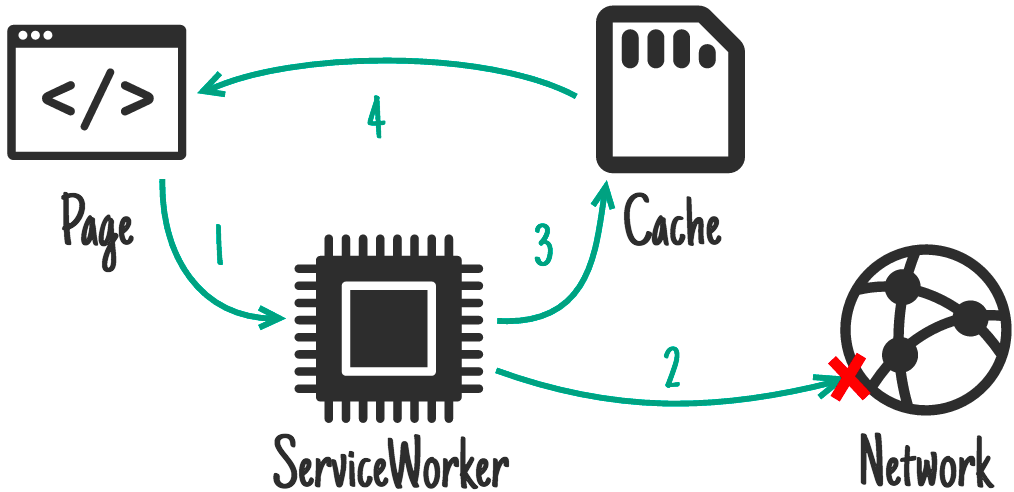
\includegraphics[width=1\textwidth]{figures/images/ss-network-falling-back-to-cache.png}
    \caption{NetworkFirst-Strategie. Quelle: The Offline Cookbook \cite{offline-cookbook}}
    \label{fig:network-first}
\end{figure}

In Zeile 35 wird definiert welche Dateien, neben den von Webpack erstellten Dateien, 
gecached werden sollen. Das sind in diesem Fall alle Daten und Dateien, die durch Netzwerkanfragen an 
das CMS geladen werden. Diese Anfragen haben den gemeinsamen Namespace \texttt{/api/} und 
können dadurch mit dem regulären Ausdruck \texttt{/.*\textbackslash/api\textbackslash/.*/} erfasst werden.
Mit der Option \texttt{handler} wird eine Caching-Strategie gewählt. Workbox bietet hier die Möglichkeit
zwischen fünf verschiedenen, vordefinierten Handler-Klassen zu wählen \cite{workbox-strategies}. 
Die Strategie der Klasse \texttt{NetworkFirst} beruht darauf, dass die Anfrage zuerst an das Netzwerk
gestellt wird. Ist dieses nicht erreichbar, wird auf die letzte Version im Cache zurückgegriffen. 
Ist ein Netzwerkzugriff erfolgreich, wird auch immer die Version im Cache durch diese Version ersetzt.
\autoref{fig:network-first} visualisiert diese Strategie. \todo{Strategie vielleicht nochmal überarbeiten}
